\section{Results}

Hereafter we list the messages peers exchange in Multipong and their
size\footnote{the size shown in the table has to be intended as ``greater or
equal than''}:

\begin{table}[H]
  \centering
  \begin{tabular}{cc}
    \textbf{\textit{Message}} & \textbf{\textit{Size [B]}} \\
    \hline
    \texttt{ARE\_YOU\_HOST} & 60 \\
    \hline
    \texttt{AVAILABLE} & 100 \\
    \hline
    \texttt{CANCEL} & 56 \\
    \hline
    \texttt{DISCOVERY} & 82 \\
    \hline
    \texttt{JOIN} & 54 \\
    \hline
    \texttt{KNOWN\_HOSTS} & 90 \\
    \hline
    \texttt{STARTING} & 187 \\
    \hline
    \texttt{TELL\_IP} & 57 \\
    \hline
    \texttt{BALL\_INFO} & 143 \\
    \hline
    \texttt{AYA} & 66 \\
    \hline
    \texttt{ACK} & 3 \\
    \hline
  \end{tabular}
  \caption{Messages size}
  \label{tab:sizes}
\end{table}

The average power consumption and Wi-Fi Direct traffic can be seen in Figures
\ref{fig:energy} and .

\begin{figure}[H]
  \centering
  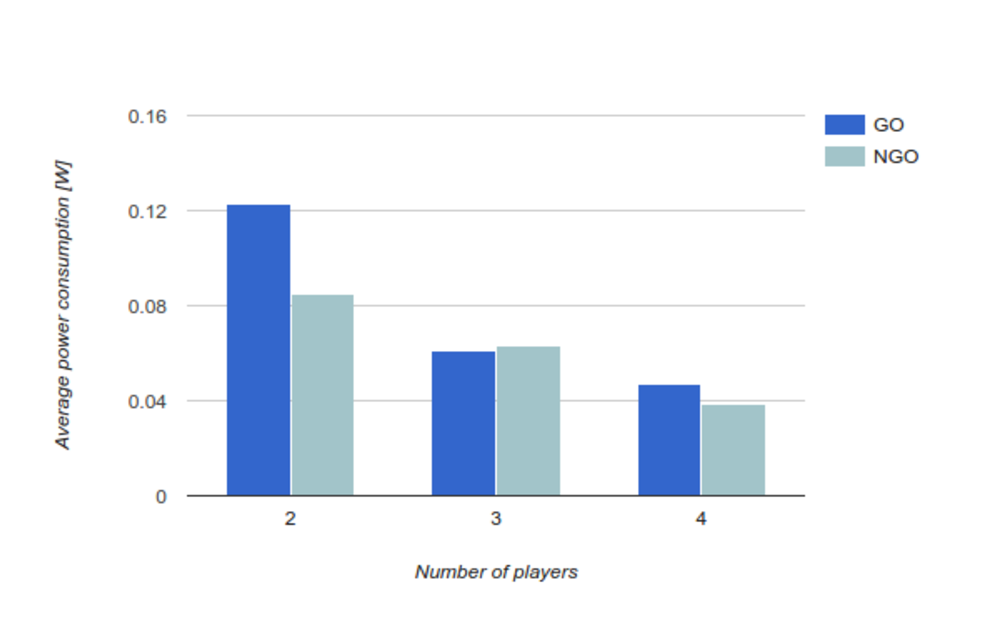
\includegraphics[width=.6\columnwidth]{img/energy.eps}
  \caption{Energy consumption comparison}
  \label{fig:energy}
\end{figure}

% TODO: Network traffic --
% TODO: 2 - 4 players comparison
% TODO: Explain why sometimes NGO > GO

% TODO: Power consumption is too variable: PowerTutor, network instability,
%       touching the screen impacts on power consumption
